\documentclass[a5paper,10pt,twoside,openany]{memoir}

% ============================================================
% A5 BOOKLET PRINTED ON FOLDED A4 SHEETS
% ============================================================
% The content is laid out as portrait A5 pages. In print mode,
% the booklet package places two A5 pages on each landscape A4
% side and rearranges the page order for folding and stapling.
%
% Recommended printer settings:
%   Paper size: A4
%   Orientation: Landscape
%   Duplex: On
%   Flip/bind: Short edge
%   Scaling: Actual size / 100 percent
% ============================================================

\newsavebox{\FrontImgBox}
\newlength{\FrontClip}

% ====== Fonts and language support ======
\usepackage[T1]{fontenc}
\usepackage[utf8]{inputenc}
\usepackage{microtype}
\ifdefined\screenproof
  % MiKTeX's screen-proof route can encounter non-scalable font
  % instances while shipping memoir pages. Protrusion remains active.
  \microtypesetup{expansion=false}
\fi
% Latin Modern is fully scalable in both screen-proof and booklet output.
\usepackage{lmodern}
\usepackage[scaled]{helvet}

% ====== Graphics, colour, columns, and boxes ======
\usepackage{float}
\usepackage{graphicx}
\usepackage{eso-pic}
\usepackage[dvipsnames]{xcolor}
\usepackage{tikz}
\usepackage{tikzpagenodes}
\usetikzlibrary{
  calc,
  decorations.text,
  fadings,
  patterns,
  positioning,
  shapes.geometric
}

\usepackage{multicol}
\setlength{\columnsep}{5mm}
\setlength{\columnseprule}{0.2pt}

\usepackage{wrapfig}
\usepackage{caption}
\captionsetup{
  font=small,
  labelfont=bf
}
\captionsetup[figure]{
  labelformat=empty
}

\usepackage{lettrine}
\usepackage[many]{tcolorbox}
\usepackage{xparse}
\usepackage{contour}
\usepackage{pgfplots}
\pgfplotsset{
  width=9cm,
  compat=1.9
}

\usepackage{ifpdf}
\usepackage{todonotes}

% ====== True A5 page layout ======
% A5 is 148.5 mm wide by 210 mm high.
\settypeblocksize{178mm}{116mm}{*}
\setlrmarginsandblock{17mm}{15.5mm}{*}
\setulmarginsandblock{16mm}{16mm}{*}
\setheadfoot{12pt}{22pt}
\setheaderspaces{*}{6mm}{*}
\checkandfixthelayout

\raggedbottom

% ====== Booklet output switch ======
% Use \bookletprinttrue for a print-ready landscape A4 PDF.
% Use \bookletprintfalse for a normal sequential portrait A5 PDF.
\newif\ifbookletprint
\ifdefined\screenproof
  \bookletprintfalse
\else
  \bookletprinttrue
\fi

% The booklet package must be loaded after the memoir page layout.
\ifbookletprint
  \usepackage[print,1to1]{booklet}
\else
  \usepackage[noprint,1to1]{booklet}
\fi

% Source page: portrait A5.
% Target sheet: landscape A4.
\source{\magstep0}{148.5mm}{210mm}
\target{\magstep0}{297mm}{210mm}

% Each signature contains up to 16 A5 pages.
% Blank pages are added automatically when required.
\pagespersignature{16}

\ifpdf
  \setpdftargetpages

  % memoir resets the PDF page size at begin-document, so set
  % the physical output size again after memoir has finished.
  \ifbookletprint
    \AtBeginDocument{%
      \pdfpagewidth=297mm
      \pdfpageheight=210mm
    }
  \fi
\else
  \setdvipstargetpages
\fi

% Optional centre-fold guide.
% Change 0pt to 0.3pt to print a faint folding line.
\setlength{\pagesepwidth}{0pt}
\setlength{\pageseplength}{190mm}
\setlength{\pagesepoffset}{10mm}

\tcbset{
  colback=black!2,
  colframe=black!40,
  boxsep=4pt,
  left=6pt,
  right=6pt,
  top=6pt,
  bottom=6pt,
  sharp corners
}

% ====== Headings and bylines ======
\setsecheadstyle{\Large\bfseries\sffamily}
\setsubsecheadstyle{\normalsize\bfseries\sffamily}
\setsubsubsecheadstyle{\normalsize\itshape}

\newcommand{\kicker}[1]{%
  \textsf{\bfseries\small\color{Gray}#1}%
}

\newcommand{\headline}[1]{%
  \textsf{%
    \bfseries
    \fontsize{24}{26}\selectfont
    #1%
  }%
}

\newcommand{\deck}[1]{%
  \textsf{\normalsize\itshape #1}%
}

\newcommand{\byline}[1]{%
  \textsf{\small\color{Gray} Af #1}%
}

% ====== Image fading ======
\tikzfading[
  name=image fade,
  inner color=transparent!50,
  outer color=transparent!100
]

% ====== Text outline ======
\contourlength{0.9pt}
\contournumber{32}

\newcommand{\ow}[2][black]{%
  \contour{#1}{\textcolor{white}{#2}}%
}

\newcommand{\owthin}[2][black]{%
  \begingroup
  \contourlength{0.6pt}%
  \contour{#1}{\textcolor{white}{#2}}%
  \endgroup
}

% ====== Page banner and folio ======
\makepagestyle{newspaper}

\makeoddhead{newspaper}
  {\textsf{\scriptsize Den Rullende Sten}}
  {}
  {\textsf{\scriptsize Sponsoreret af Det Glemte Akademi}}

\makeevenhead{newspaper}
  {\textsf{\scriptsize Sponsoreret af Det Glemte Akademi}}
  {}
  {\textsf{\scriptsize Den Rullende Sten}}

\makeoddfoot{newspaper}
  {}
  {\textsf{\scriptsize\thepage}}
  {}

\makeevenfoot{newspaper}
  {}
  {\textsf{\scriptsize\thepage}}
  {}

\makeheadrule{newspaper}{\textwidth}{0.4pt}
\pagestyle{newspaper}

% ====== Pull quote environment ======
\newenvironment{pullquote}
  {%
    \begin{tcolorbox}[
      enhanced,
      breakable
    ]
    \itshape
    \large
  }
  {%
    \end{tcolorbox}
  }

% ====== Sidebar settings ======
\newcounter{sidebarlines}
\setcounter{sidebarlines}{14}
\setlength{\sidebarwidth}{0.42\columnwidth}

\newcommand{\godentry}[5]{%
  % #1 = placering
  % #2 = titel
  % #3 = billedfil
  % #4 = side l/r
  % #5 = tekst

  \begin{wrapfigure}{#4}{0.24\columnwidth}
    \vspace{-8pt}
    \centering
    \includegraphics[
      width=0.20\columnwidth
    ]{#3}
    \vspace{-12pt}
  \end{wrapfigure}

  \subsection*{#1. #2}

  #5

  \par\medskip
}

% ====== Utilities ======
\newcommand{\separator}{%
  \par
  \noindent
  {\color{black!40}\rule{\textwidth}{0.4pt}}
  \par
}

% ====== Front feature image ======
% Usage:
% \FrontFeatureImage
%   {image}
%   {kicker}
%   {headline}
%   {deck}
%   {credit}

\newcommand{\FrontFeatureImage}[5]{%
  % Typeset and measure the image.
  \sbox{\FrontImgBox}{%
    \includegraphics[
      width=0.94\textwidth
    ]{#1}%
  }%

  % Total scaled image height.
  \dimen0=\dimexpr
    \ht\FrontImgBox+
    \dp\FrontImgBox
  \relax

  % Maximum image height on an A5 page.
  \dimen2=.70\textheight

  % Select the visible height.
  \ifdim\dimen0>\dimen2
    \setlength{\FrontClip}{\dimen2}%
  \else
    \setlength{\FrontClip}{\dimen0}%
  \fi

  \begin{tikzpicture}
    % Image frame coordinates.
    \coordinate (TL) at (0,0);
    \coordinate (TR) at (\textwidth,0);
    \coordinate (BL) at (0,-\FrontClip);
    \coordinate (BR) at (\textwidth,-\FrontClip);

    % Image.
    \begin{scope}
      \clip (TL) rectangle (BR);

      \node[
        anchor=north west,
        inner sep=0pt,
        path fading=image fade,
        fit fading=false
      ] at (TL) {%
        \usebox{\FrontImgBox}%
      };
    \end{scope}

    % Dark overlay for text legibility.
    \begin{scope}
      \clip (TL) rectangle (BR);

      \fill[
        black,
        opacity=0.30,
        path fading=image fade
      ]
      (BL) rectangle (TR);
    \end{scope}

    % Headline stack.
    \node[
      anchor=south west,
      xshift=1em,
      yshift=1em,
      align=left,
      text width=.75\textwidth
    ] at (BL) {%
      \sffamily

      \if\relax\detokenize{#2}\relax
      \else
        {%
          \owthin[black!85]{%
            \textsf{\bfseries\small #2}%
          }%
        }\\[0.15em]
      \fi

      {%
        \ow{%
          \bfseries
          \resizebox{\textwidth}{!}{#3}%
        }%
      }\\[0.2em]

      {%
        \owthin{%
          \large
          \itshape
          #4%
        }%
      }%
    };

    % Image credit.
    \node[
      anchor=south east,
      xshift=-1em,
      yshift=1em
    ] at (BR) {%
      \sffamily
      \small
      \owthin[black!85]{#5}%
    };
  \end{tikzpicture}%
}

% ====== Information box ======
\newenvironment{infobox}[1]
  {%
    \begin{tcolorbox}[
      title=\textsf{\bfseries #1},
      colback=black!3,
      colframe=black!65,
      fonttitle=\small,
      fontupper=\small,
      boxsep=4pt,
      left=5pt,
      right=5pt,
      top=5pt,
      bottom=5pt,
      sharp corners
    ]
  }
  {%
    \end{tcolorbox}
  }

\newcommand{\paragraf}[1]{%
  \par
  \medskip
  \noindent
  \textbf{\S#1:}%
}

\begin{document}

% ============================================================
% FRONT PAGE
% ============================================================

\begin{center}
  
\includegraphics[
    width=0.98\textwidth
  ]{Logo.png}
\end{center}

\begin{center}
  {\Large\sffamily Udgave 136}
\end{center}

\FrontFeatureImage
  {assets/royal/Aurelia Fjendebane.jpg}
  {Kejserinde Aurelia er død}
  {DEN RØDE TRONE STÅR TOM}
  {Syndicatet mistænkes, mens fire parter ruster til borgerkrig}
  {}

\vspace{.75\baselineskip}

\newpage

% ====== Lead story ======
\par\medskip
\headline{KEJSERINDEN ER DØD\\ BORGERKRIGEN BEGYNDER}
\par\medskip
\deck{Aurelia døde efter sit besøg i A'kastin. Nu marcherer hære mod Nordland, mens en ubekræftet mistanke retter sig mod terrorgruppen Syndicatet.}
\par\medskip
\byline{Redaktionen}
\medskip

\lettrine[lines=3,lhang=0.1,loversize=0.05]{K}{ejserinde}
Aurelia Fjendebane er død, og med hende er den sidste ubestridte regent af Den Røde Trone forsvundet. Dødsbudskabet kom kort efter hendes besøg i A'kastin, hvor hun havde vist sig blandt konger, præster og soldater, men dog beskyttet af Den Royale Garde.

\begin{wrapfigure}[23]{r}{0.43\columnwidth}
\vspace{4pt}
\begin{infobox}{DET VED VI}
\begin{itemize}
\setlength{\itemsep}{0.25em}
\item Aurelia døde efter sit besøg i A'kastin.
\item Dødsårsagen er ikke offentligt fastslået.
\item Syndicatet nævnes som mulig bagmand, men ingen beviser er fremlagt.
\item Conrad Fjendebane marcherer mod Nordland med en hær.
\item Talia, Severin og Ismarelda fremsætter hver deres krav til rigets fremtid.
\end{itemize}
\end{infobox}
\end{wrapfigure}

Hoffet har endnu ikke fremlagt en dødsårsag. Der er heller ikke offentliggjort et tidspunkt, et gerningssted eller navnet på en mistænkt. Alligevel har nyheden allerede sat hære i bevægelse.

Conrad Fjendebane, der i årevis blev regnet for død ved Sydporten, er vendt tilbage i spidsen for en hær. Hans mål er Nordland og Den Røde Trone. Samtidig nægter hans egne børn og Ismarelda Vinterkrone at anerkende hans ret til at herske.

\subsection*{Dødsbuddet efter A'kastin}

Aurelias rejse til A'kastin er det sidste sikre holdepunkt i fortællingen om hendes liv. Hun blev set blandt flere af Kalishs magtfulde skikkelser og forlod siden besøget. Derefter kom meldingen om hendes død.

Det er endnu uklart, om hun døde under hjemrejsen, mens hun stadig var i A'kastin eller et helt tredje sted. Netop manglen på en officiel forklaring har gjort hvert hul i tidslinjen til grobund for rygter og konspirations teorier.

Nogle peger på striden om guddommelig magt i A'kastin. Andre peger på kejserfamiliens egne fjender. Det alvorligste rygte nævner dog den skjulte terrorgruppe kendt som Syndicatet.

\subsection*{Syndicatets skygge}

Ingen myndighed har fremlagt beviser for, at Syndicatet dræbte Aurelia. Den Rullende Sten kan heller ikke bekræfte, at gruppens medlemmer befandt sig nær kejserinden. Mistanken skal derfor behandles som netop en mistanke.

Men teorien spreder sig af en grund. Det er ingen hemmelighed at Aurelia var en af spidskandidaterne til blive ophøjet som en ny gudinde. Derfor er det ikke utænkeligt at denne gruppe som er modstander af alle guder, ville gøre deres for at stoppe hende.

Det afgørende spørgsmål er derfor, hvem der kunne komme tæt nok på Aurelia efter besøget i A'kastin. Indtil hoffet åbner sine arkiver må dette være hen i det uvisse, men nogen peger på at det kunne være Dorian Vinterkrone, for at give hans bedstemor en mulighed for at blive kejserinde.

\subsection*{Den døde kejsersøn vender tilbage}

Mens mistanken samler sig om Aurelias død, har Conrad Fjendebane gjort sit krav umuligt at overse.

Conrad er søn af Erik II og blev meldt død efter slaget ved Sydporten. Nu hævder han, at beretningen var falsk, og at han overlevede. Under Imperiets symbol fører han en blandet hær af mennesker, elvere, dværge og orkere mod Nordland for at tage Den Røde Trone, som per lov er hans.

Talia og Severin Fjendebane påstår, at deres far virkelig døde ved Sydporten. Ifølge dem er den skikkelse, der nu kalder sig Conrad, et gespenst vækket til live af den nederdrægtige Hrothgar. Den mystiske ork blev set ved A'kastin i sommer, kort før Conrad igen viste sig. Dette ville selvfølgelig gøre Conrads krav på tronen ugyldig, og under normale omstændigheder ville kronen tilfalde den næste arving.

Ingen undersøgelse har afgjort, om Conrad er levende, genopstået eller noget helt tredje.

\subsection*{Børnene vælger hver sin fremtid}

Conrads børn står sammen om mistanken mod deres far, men ikke om, hvad der bør erstatte ham.

\textbf{Talia Fjendebane} voksede op i Permersland og har samlet kræfter omkring et radikalt opgør med selve den royale linje. Hun vil ikke blot udskifte personen på tronen. Hendes tilhængere vil bryde den gamle kejserfamilies magt og skabe et andet Imperium af resterne, et hun påstår er eget af folket. Dette gør naturligt at mange ser hende som en ustabil kandidat, især da hun opgav retten til at arve kronen og vidergive den til Aurelia.

\textbf{Severin Fjendebane} blev derimod opdraget i Kelllwan Kirken. Han hævder som Conrads førstefødte sin egen arveret, men ser tronen som redskab for et religiøst enevælde. Mange frygter at han vil placere Kelllwans messias på tronen, hvilket ville medfører ustabilitet, og eksperter ser at dette kunne vælte Salezstand og Rosenborg som handels-centrummer, hvis andre religioner ikke er velkommende. 

De to arvinger kan altså være enige om, at Conrad ikke længere er deres far. Men Severin mener at Talia er en front for Syndicatet, som har haft rødder i Permersland, mens Talia mener at Severin opgav alle krav på tronen da han viede sig selv til Kirken.

\subsection*{Vinterkronens lovkrav}

Den fjerde part er \textbf{Ismarelda Vinterkrone}, grankusine til Erik II. Mens Aurelia befandt sig i A'kastin, overtog Ismarelda pladsen som regent, da pladsen lovligt faldt til hende. Efter dødsbudskabet hævder hun, at dette ansvar og hendes plads i slægten gør hende til den eneste lovlige arving.

Denne påstand er heller ikke uden vægt. Hvis Conrad viser sig at være et gespenst som blev genoplivet af Hrothgar, så er der et argument i at Conrads børn allerede har gjort afkast på tronen, og derfor ikke kan være retmæssige arvinger. I såfald, vil Ismarelda være den næste arving\footnote{Det forventes ikke at man vil skifte navnenet på Fjend til Vinter}.

Hendes støtter fremhæver, at hun allerede har båret rigets ansvar, og derfor også han den nødvendige erfaring for at opretholde fred.

Vinterkronens stærkeste indflydelse findes i Salezstand, hvor hendes barnebarn Dorian Vinterkrone allerede har lagt meget arbejde i at sprede hans indflydelse. Det gør hende vanskelig at ignorere, selv hvis Conrad når Nordland først.

\subsection*{Nordland kan blive den første front}

Conrads fremmarch gør Nordland til borgerkrigens umiddelbare brændpunkt. Det er tydeligt at alle partner på nuværende tidspunkt undgår A'kastin, I et håb om at bevare deres styrker. Men hvis Conrad indtager Den Røde Trone vil de andre parter måske begynde at rekrutere eventyrer hvis loyalitet ikke kan verificeres.

Men krigen afgøres næppe alene der. Talia kan trække på utilfredsheden i Permersland, Severin på kirken og Ismarelda på de dele af adelen, der foretrækker lov og kontinuitet.

Borgerne bør være varsomme med rygter og skråsikre bekendtgørelser. Hold øje med troppebevægelser, lukkede veje og krav om troskabsed.

På de følgende sider bringer vi kejserfamiliens stamtræ og en oversigt over de fire parter.

% ============================================================
% ROYAL FAMILY TREE - TWO-PAGE FEATURE
% ============================================================

% Two-page succession feature for Den Rullende Sten.
% Solid dark-red lines are direct named descent. The solid blue connector is a
% documented collateral line, abbreviated here to fit the newspaper page.

\definecolor{ImperialRed}{HTML}{711A22}
\definecolor{ImperialDarkRed}{HTML}{3A1116}
\definecolor{ImperialGold}{HTML}{BF8B2E}
\definecolor{ImperialCream}{HTML}{F5EEDC}
\definecolor{ImperialInk}{HTML}{24191A}
\definecolor{RebelRed}{HTML}{9B2F25}
\definecolor{ChurchGold}{HTML}{B68A26}
\definecolor{WinterBlue}{HTML}{294B6D}

\newcommand{\PortraitCrop}[3]{%
  \includegraphics[
    width=#1,
    height=#2,
    keepaspectratio,
    trim=45 250 45 0,
    clip
  ]{#3}%
}

% Keep portrait and faction mark optically centred on a shared midline.
% #1/#2 = portrait box, #3 = portrait file, #4 = mark, #5 = gap.
\newcommand{\PortraitLockup}[5]{%
  \makebox[\linewidth][c]{%
    \begin{tabular}{@{}c@{\hspace{#5}}c@{}}
      \raisebox{-0.5\height}{\PortraitCrop{#1}{#2}{#3}} &
      \raisebox{-0.5\height}{#4}
    \end{tabular}%
  }%
}

\newcommand{\ImperialMark}{%
  
\includegraphics[width=13mm]{assets/royal/Imperiet.jpg}%
}

\newcommand{\TaliaMark}{%
  
\includegraphics[width=13mm]{assets/royal/Talia-rebel-crown.png}%
}

\newcommand{\SeverinMark}{%
  
\includegraphics[width=13mm]{assets/royal/Severin-church-crown.png}%
}

\newcommand{\IsmareldaMark}{%
  
\includegraphics[width=13mm]{assets/royal/Ismarelda-winter-crown.png}%
}

\tikzset{
  family card/.style={
    draw=ImperialGold,
    line width=0.7pt,
    fill=white,
    rounded corners=1.2mm,
    inner sep=1.5mm,
    align=center
  },
  claim card/.style={
    draw=ImperialGold,
    line width=0.75pt,
    fill=white,
    rounded corners=1.2mm,
    inner sep=1.8mm,
    align=left
  },
  family line/.style={
    draw=ImperialDarkRed,
    line width=0.85pt
  },
  archive branch/.style={
    draw=WinterBlue,
    line width=1.05pt
  }
}

% ============================================================
% PAGE ONE - THE NEW SUCCESSION TREE
% ============================================================

% Always begin this feature on an even-numbered logical newspaper page.
\clearpage
\ifodd\value{page}
  % If a parity page is needed, use it to thank the academy's patron.
  \thispagestyle{empty}
  \vspace*{-\topskip}
  \noindent
  \begin{tikzpicture}[x=1mm,y=1mm,baseline=(thankbase)]
    \path[use as bounding box] (0,0) rectangle (116,-178);
    \coordinate (thankbase) at (0,0);

    \draw[ImperialDarkRed,line width=1.2pt] (-18,10) rectangle (118,-188);
    \draw[ImperialGold,line width=0.45pt] (-16,8) rectangle (116,-186);

    \node[anchor=north west,align=left,text width=110mm]
      at (1,-1) {%
        {\sffamily\bfseries\scriptsize\color{ImperialRed}
         DET GLEMTE AKADEMI TAKKER}\par
        \vspace{0.4mm}
        {\sffamily\bfseries\fontsize{17}{18}\selectfont
         KONG DORIAN VINTERKRONE}\par
        \vspace{0.5mm}
        {\sffamily\small\itshape\color{black!66}
         Konge af A'kastin}%
      };

    \fill[ImperialDarkRed] (1,-25) rectangle (113,-28);

    \node[anchor=center] at (30,-91) {%
      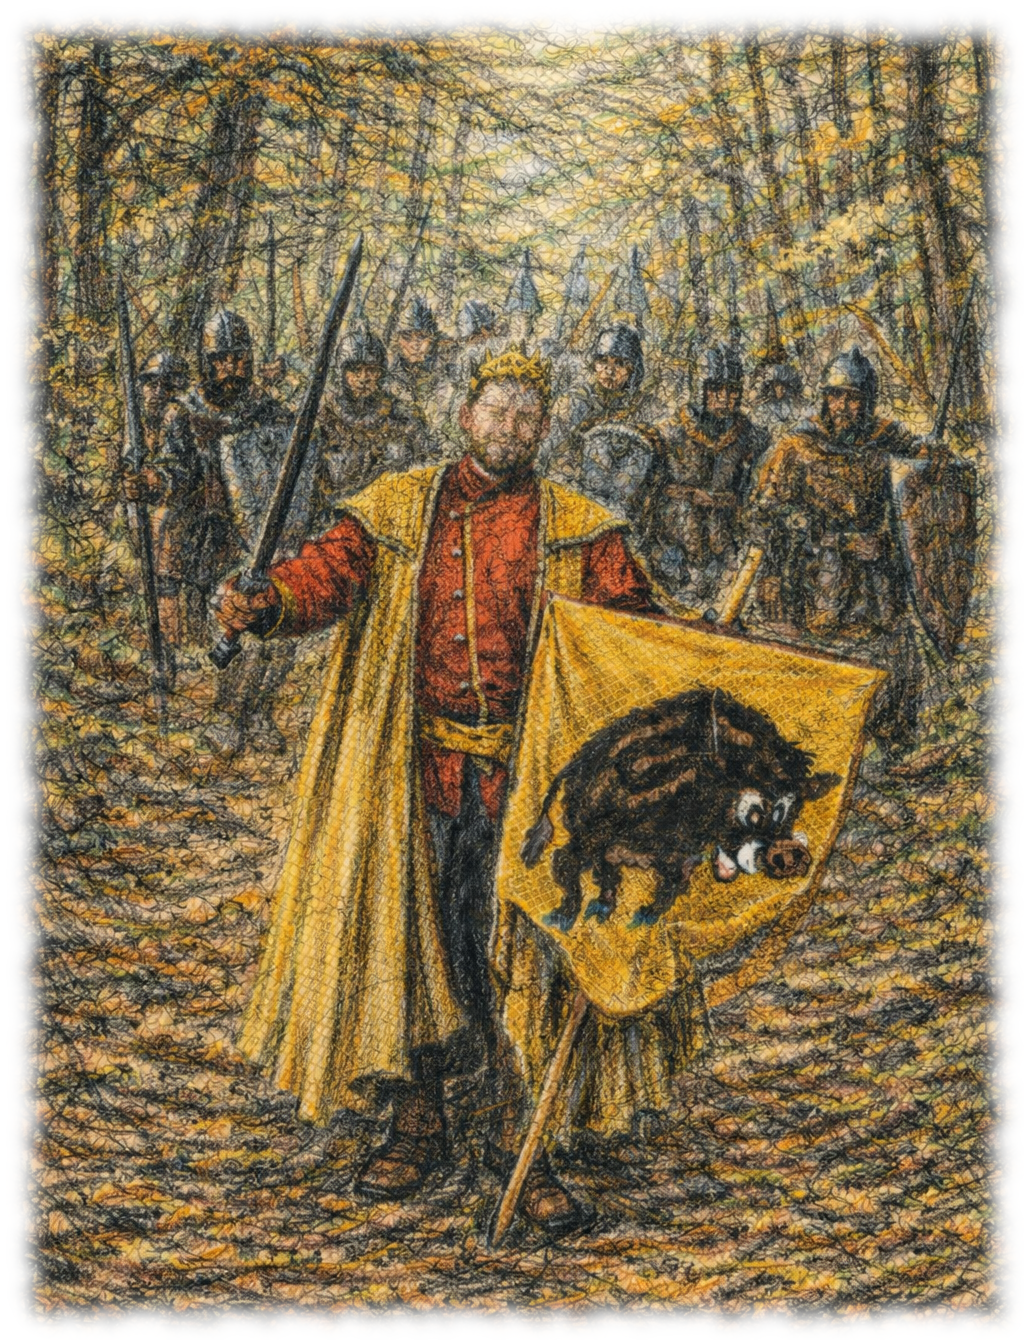
\includegraphics[height=103mm]{assets/royal/Kong Dorian.png}%
    };

    \node[
      anchor=north west,
      text width=40mm,
      align=center,
      fill=white,
      draw=ImperialGold,
      line width=0.8pt,
      rounded corners=1.2mm,
      inner sep=2.4mm
    ] at (69,-38) {%
      
\includegraphics[height=45mm]{assets/royal/vinterkroneSkjold.png}\par
      \vspace{1.4mm}
      {\sffamily\bfseries\scriptsize\color{WinterBlue}
       FOR STØTTEN TIL AKADEMIET}\par
      \vspace{1.2mm}
      {\sffamily\fontsize{7.2}{8.4}\selectfont\color{ImperialInk}
       Det Glemte Akademi takker Kong Dorian Vinterkrone for hans støtte til vores arbejde.\par
       \vspace{1.1mm}
       Hans hjælp holder blæk i husene, papir i trykpressen og budbringere
       på vejene, så nyheder og velunderbyggede rygter fortsat kan nå
      borgerene af Kalish.}\par
      \vspace{1.5mm}
      {\color{ImperialGold}\rule{29mm}{0.45pt}}\par
      \vspace{0.8mm}
      {\sffamily\bfseries\fontsize{6.7}{7.4}\selectfont
       MED TAKNEMMELIGHED\par
       REDAKTIONEN PÅ DEN RULLENDE STEN}%
    };

    \node[
      anchor=south west,
      align=center,
      text width=107mm,
      fill=ImperialDarkRed,
      text=white,
      inner sep=2.3mm
    ] at (1,-176) {%
      {\sffamily\bfseries\scriptsize
       Vi er stolte af at kunne sige at vi får støtte fra en sand helt blandt kujoner.}\par
      \vspace{0.5mm}
      {\sffamily\fontsize{6.8}{7.8}\selectfont
       Redaktionen håber at Kong Dorian får et langt og lykkeligt liv!}%
    };
  \end{tikzpicture}\par
  \clearpage
\fi
\thispagestyle{empty}
\vspace*{-\topskip}
\noindent

\begin{tikzpicture}[x=1mm,y=1mm,baseline=(pagebaseone)]
  \path[use as bounding box] (0,0) rectangle (116,-178);
  \coordinate (pagebaseone) at (0,0);

  \draw[ImperialDarkRed,line width=1.2pt] (-18,10) rectangle (118,-188);
  \draw[ImperialGold,line width=0.45pt] (-16,8) rectangle (116,-186);
  \coordinate (NW) at (0,0);

  \node[anchor=north west,align=left,text width=105mm]
    at ([xshift=1mm,yshift=-1mm]NW) {%
      {\sffamily\bfseries\scriptsize\color{ImperialRed}
       EKSTRA: SLAGET OM ARVEFØLGEN}\par
      \vspace{0.3mm}
      {\sffamily\bfseries\fontsize{18}{19}\selectfont
       DEN RØDE TRONE STÅR TOM}\par
      \vspace{0.5mm}
      {\sffamily\small\itshape\color{black!70}
       Aurelia er død.\\ Conrad er vendt tilbage.\\ Tre andre
       tronkrav nægter at bøje sig for ham.}%
    };



  \node[
    anchor=north west,
    text width=111mm,
    align=center,
    fill=ImperialDarkRed,
    text=white,
    inner xsep=1mm,
    inner ysep=1.1mm
  ] at ([xshift=1mm,yshift=-25mm]NW) {%
    \sffamily\bfseries\fontsize{6.6}{7.3}\selectfont
  };

  \node[
    family card,
    text width=29mm,
    minimum height=25mm
  ] (erik) at ([xshift=58mm,yshift=-46mm]NW) {%
    
\includegraphics[width=16mm,height=13mm,keepaspectratio]{assets/royal/Erik Fjendebane.png}\\[-0.7mm]
    {\sffamily\bfseries\scriptsize KEJSER ERIK II}\\[-0.3mm]
    {\sffamily\fontsize{6.2}{6.9}\selectfont\color{black!58}
     Faldt ved Sydporten}%
  };

  \coordinate (siblingsplit) at ([yshift=-5mm]erik.south);
  \draw[family line] (erik.south) -- (siblingsplit);
  \draw[family line] ([xshift=-30mm]siblingsplit) -- ([xshift=30mm]siblingsplit);

  \node[
    family card,
    text width=38mm,
    minimum height=38mm
  ] (conrad) at ([xshift=28mm,yshift=-85mm]NW) {%
    \PortraitLockup{22mm}{20mm}{assets/royal/Conrad Fjendebane.png}{\ImperialMark}{2mm}\\[1mm]
    {\sffamily\bfseries\small CONRAD FJENDEBANE}\\[-0.2mm]
    {\sffamily\fontsize{6.5}{7.3}\selectfont\color{black!62}
     Erik II's søn som marcherer mod Nordland\\
     \color{ImperialRed}\bfseries Levende eller Hrothgars gespenst?}%
  };

  \node[
    family card,
    draw=ImperialRed,
    line width=1.1pt,
    text width=38mm,
    minimum height=38mm
  ] (aurelia) at ([xshift=88mm,yshift=-85mm]NW) {%
    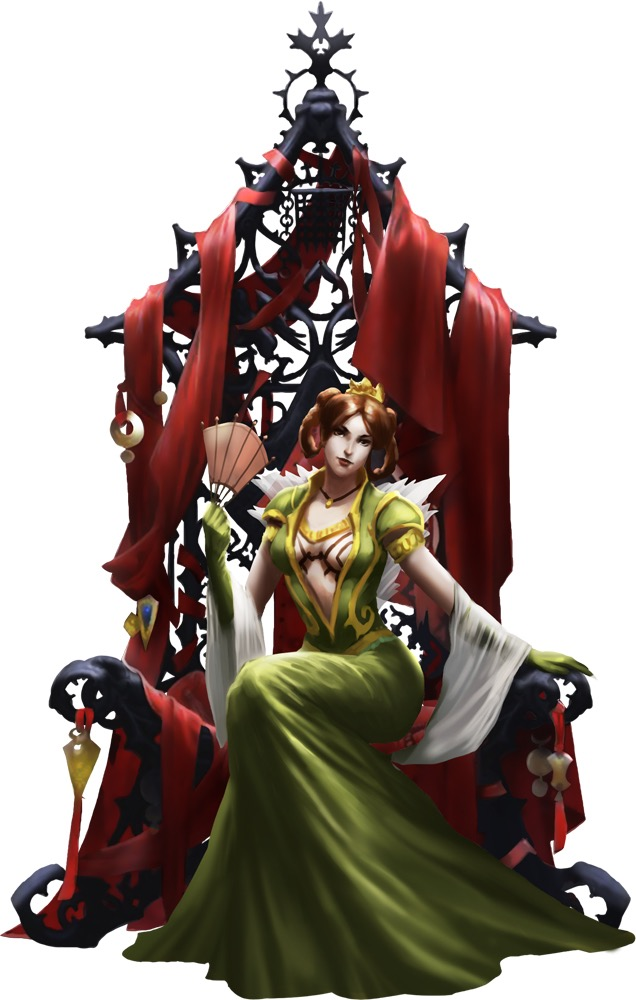
\includegraphics[width=27mm,height=23mm,keepaspectratio]{assets/royal/Aurelia Fjendebane.jpg}\\[-0.5mm]
    {\sffamily\bfseries\small KEJSERINDE AURELIA}\\[-0.2mm]
    {\sffamily\fontsize{6.7}{7.4}\selectfont\color{ImperialRed}\bfseries
     HVEM DRÆBTE KEJSERINDEN?}%
  };

  \draw[family line] ([xshift=-30mm]siblingsplit) |- (conrad.north);
  \draw[family line] ([xshift=30mm]siblingsplit) |- (aurelia.north);

  \coordinate (childsplit) at ([yshift=-5mm]conrad.south);
  \draw[family line] (conrad.south) -- (childsplit);
  \draw[family line] ([xshift=-14.5mm]childsplit) -- ([xshift=14.5mm]childsplit);

  \node[
    family card,
    draw=RebelRed,
    text width=30mm,
    minimum height=41mm
  ] (talia) at ([xshift=13.5mm,yshift=-132mm]NW) {%
    \PortraitLockup{16mm}{17mm}{assets/royal/Talia Fjendebane.png}{\TaliaMark}{1mm}\\[1mm]
    {\sffamily\bfseries\scriptsize TALIA FJENDEBANE}\\[-0.1mm]
    {\sffamily\fontsize{6.1}{6.8}\selectfont\color{black!62}
     Opvokset i Permersland\\
     \color{RebelRed}\bfseries Radikalt opgør mod blodretten}%
  };

  \node[
    family card,
    draw=ChurchGold,
    text width=30mm,
    minimum height=41mm
  ] (severin) at ([xshift=48.5mm,yshift=-132mm]NW) {%
    \PortraitLockup{16mm}{17mm}{assets/royal/Severin Fjendebane.png}{\SeverinMark}{1mm}\\[1mm]
    {\sffamily\bfseries\scriptsize SEVERIN FJENDEBANE}\\[-0.1mm]
    {\sffamily\fontsize{6.1}{6.8}\selectfont\color{black!62}
     Opvokset i Kelllwan Kirken\\
     \color{ChurchGold!80!black}\bfseries Støttet af Kelllwans Messias}%
  };

  \draw[family line] ([xshift=-14.5mm]childsplit) |- (talia.north);
  \draw[family line] ([xshift=14.5mm]childsplit) -| (severin.north);

  \node[
    family card,
    draw=WinterBlue,
    line width=1.05pt,
    text width=39mm,
    minimum height=44mm
  ] (ismarelda) at ([xshift=90mm,yshift=-132mm]NW) {%
    \PortraitLockup{20mm}{20mm}{assets/royal/Ismarelda Vinterkrone.png}{\IsmareldaMark}{1.5mm}\\[1mm]
    {\sffamily\bfseries\small ISMARELDA VINTERKRONE}\\[-0.1mm]
    {\sffamily\fontsize{6.1}{6.8}\selectfont\color{black!62}
     Grankusine til Erik II\\
     Familien har størst indflydelse i Salezstand.\\
     \color{WinterBlue}\bfseries Kalder sig eneste\\lovlige arving}%
  };

  \draw[archive branch] (erik.east) -- ++(40mm,0) |- (ismarelda.east);
  \node[
    anchor=west,
    rotate=90,
    inner sep=0.5mm
  ] at ([xshift=39mm,yshift=-40mm]erik.east) {%
    \sffamily\fontsize{5.8}{6.4}\selectfont\color{WinterBlue}
    Sidegren (forkortet for læsernes skyld)%
  };

  \node[
    anchor=south west,
    align=left,
    text width=107mm,
    fill=ImperialDarkRed,
    text=white,
    inner sep=2mm
  ] at ([xshift=1mm,yshift=-176mm]NW) {%
    {\sffamily\bfseries\scriptsize BORGERKRIG OM DEN RØDE TRONE!}\par
    \vspace{0.4mm}
    {\sffamily\fontsize{6.6}{7.6}\selectfont
     Conrad hævder, at han overlevede Sydporten. Hans egne børn siger,
     at faderen døde og siden blev vækket af Hrothgar. Nu kræver både
     børnene og Vinterkrone-sidegrenen retten til at forme det næste imperium.}%
  };
\end{tikzpicture}\par

\clearpage

% ============================================================
% PAGE TWO - FOUR COMPETING CLAIMS
% ============================================================

\thispagestyle{empty}
\vspace*{-\topskip}
\noindent

\begin{tikzpicture}[x=1mm,y=1mm,baseline=(pagebasetwo)]
  \path[use as bounding box] (0,0) rectangle (116,-178);
  \coordinate (pagebasetwo) at (0,0);

  \draw[ImperialDarkRed,line width=1.2pt] (-18,10) rectangle (118,-188);
  \draw[ImperialGold,line width=0.45pt] (-16,8) rectangle (116,-186);
  \coordinate (NW) at (0,0);

  \node[anchor=north west,align=left,text width=111mm]
    at ([xshift=1mm,yshift=-1mm]NW) {%
      {\sffamily\bfseries\scriptsize\color{ImperialRed}
       MAGTKAMPEN EFTER AURELIA}\par
      \vspace{0.3mm}
      {\sffamily\bfseries\fontsize{18}{19}\selectfont
       FIRE KRAV PÅ TRONEN}\par
      \vspace{0.5mm}
      {\sffamily\small\itshape\color{black!70}
       Borgerkrigen afgøres med kampen om Salezstand.}%
    };

  \node[
    claim card,
    text width=48mm,
    minimum height=53mm
  ] (conradclaim) at ([xshift=28mm,yshift=-59mm]NW) {%
    \PortraitLockup{22mm}{22mm}{assets/royal/Conrad Fjendebane.png}{\ImperialMark}{3mm}\par
    \vspace{0.6mm}
    {\sffamily\bfseries\fontsize{7.2}{8}\selectfont\color{ImperialRed}
     DEN TILBAGEVENDTE KEJSERSØN}\par
    {\sffamily\bfseries\small CONRAD FJENDEBANE}\par
    \vspace{0.7mm}
    {\sffamily\fontsize{6.5}{7.4}\selectfont
     \textbf{Krav:} Direkte arveret efter Erik II.\par
     \textbf{Styrke:} Blandede tropper af både elvere, orkere, dværge og mennesker.\par
     \textbf{Tvivl:} Conrad genopstod efter Hrothgar var set i A'kastin.}%
  };

  \node[
    claim card,
    draw=RebelRed,
    text width=48mm,
    minimum height=53mm
  ] (taliaclaim) at ([xshift=88mm,yshift=-59mm]NW) {%
    \PortraitLockup{22mm}{22mm}{assets/royal/Talia Fjendebane.png}{\TaliaMark}{3mm}\par
    \vspace{0.6mm}
    {\sffamily\bfseries\fontsize{7.2}{8}\selectfont\color{RebelRed}
     PERMERSLANDS OPRØRSARVING}\par
    {\sffamily\bfseries\small TALIA FJENDEBANE}\par
    \vspace{0.7mm}
    {\sffamily\fontsize{6.5}{7.4}\selectfont
     \textbf{Krav:} Conrads andet barn.\par
     \textbf{Styrke:} Samler oprørerne fra Permersland under sig.\par
     \textbf{Tvivl:} Hun har gjort det tydeligt at Kejserfamilien skal knuses.}%
  };

  \node[
    claim card,
    draw=ChurchGold,
    text width=48mm,
    minimum height=53mm
  ] (severinclaim) at ([xshift=28mm,yshift=-119mm]NW) {%
    \PortraitLockup{22mm}{22mm}{assets/royal/Severin Fjendebane.png}{\SeverinMark}{3mm}\par
    \vspace{0.6mm}
    {\sffamily\bfseries\fontsize{7.2}{8}\selectfont\color{ChurchGold!75!black}
     KELLLWANS HELLIGE ARVING}\par
    {\sffamily\bfseries\small SEVERIN FJENDEBANE}\par
    \vspace{0.7mm}
    {\sffamily\fontsize{6.5}{7.4}\selectfont
     \textbf{Krav:} Conrads førstefødte\par
     \textbf{Styrke:} Kelllwans messias støtter ham.\par
     \textbf{Tvivl:} Står for religiøst enevælde under Kelllwan.}%
  };

  \node[
    claim card,
    draw=WinterBlue,
    text width=48mm,
    minimum height=53mm
  ] (ismareldaclaim) at ([xshift=88mm,yshift=-119mm]NW) {%
    \PortraitLockup{22mm}{22mm}{assets/royal/Ismarelda Vinterkrone.png}{\IsmareldaMark}{3mm}\par
    \vspace{0.6mm}
    {\sffamily\bfseries\fontsize{7.2}{8}\selectfont\color{WinterBlue}
     DEN LOVLIGE ARVING}\par
    {\sffamily\bfseries\small ISMARELDA VINTERKRONE}\par
    \vspace{0.7mm}
    {\sffamily\fontsize{6.5}{7.4}\selectfont
     \textbf{Krav:} Overtog pladsen som regent mens Aurelia var i A'kastin.\par
     \textbf{Styrke:} Hendes barnebarn har stor indflydelse i Salezstand.\par
     \textbf{Tvivl:} Er hun blot mere af det samme?}%
  };

  \node[
    anchor=south west,
    align=left,
    text width=107mm,
    fill=ImperialDarkRed,
    text=white,
    inner sep=2mm
  ] at ([xshift=1mm,yshift=-176mm]NW) {%
    {\sffamily\bfseries\scriptsize HROTHGAR-SPØRGSMÅLET}\par
    \vspace{0.4mm}
    {\sffamily\fontsize{6.6}{7.6}\selectfont
     Conrads børn peger på, at den mystiske ork Hrothgar blev set ved
     A'kastin just en måned før Conrad kom tilbage ved Sydporten. 
     Ingen uafhængig kilde har bevist, at han vækkede
     Conrad, men Conrads tropper vil pege på en ændring af Imperiets udenrigspolitik.}%
  };
\end{tikzpicture}\par

\clearpage



% ====== Rohar advertisement ======
\begin{center}
  \begin{tcolorbox}[
    enhanced,
    breakable,
    width=0.94\textwidth,
    colback=ForestGreen!4,
    colframe=black,
    boxrule=1.4pt,
    borderline={
      0.7pt
    }{
      3pt
    }{
      ForestGreen!70!black
    },
    sharp corners,
    boxsep=2mm,
    left=5mm,
    right=5mm,
    top=4mm,
    bottom=3mm,
    overlay={
      % Top-left ornament.
      \draw[
        ForestGreen!70!black,
        line width=1.2pt
      ]
      ([xshift=2mm,yshift=-2mm]frame.north west)
      -- ++(11mm,0)
      -- ++(0,-7mm);

      % Top-right ornament.
      \draw[
        ForestGreen!70!black,
        line width=1.2pt
      ]
      ([xshift=-2mm,yshift=-2mm]frame.north east)
      -- ++(-11mm,0)
      -- ++(0,-7mm);

      % Bottom-left ornament.
      \draw[
        ForestGreen!70!black,
        line width=1.2pt
      ]
      ([xshift=2mm,yshift=2mm]frame.south west)
      -- ++(11mm,0)
      -- ++(0,7mm);

      % Bottom-right ornament.
      \draw[
        ForestGreen!70!black,
        line width=1.2pt
      ]
      ([xshift=-2mm,yshift=2mm]frame.south east)
      -- ++(-11mm,0)
      -- ++(0,7mm);
    }
  ]

    \begin{center}
      {%
        \sffamily
        \bfseries
        \small
        TRÆT AF SVAGE GUDER OG TOMME LØFTER?%
      }

      \vspace{0.15em}

      {%
        \sffamily
        \bfseries
        \fontsize{22}{24}\selectfont
        \textcolor{ForestGreen!55!black}{%
          REJS DIG FOR ROHAR!%
        }%
      }

      \vspace{0.1em}

      {%
        \sffamily
        \bfseries
        \large
        KONGEN - DEN DER KOM TILBAGE%
      }
    \end{center}

    \vspace{0.5em}

    \noindent
    \colorbox{black}{%
      \parbox{\dimexpr\linewidth-2\fboxsep\relax}{%
        \centering
        \color{white}
        \itshape
        \large

        ``Før var jeg træt og deprimeret, men så prøvede jeg
        at tilbede Rohar. Nu har jeg styrke, et formål og en
        gud, der råber gode råd gennem min økse!''

        \normalfont
        \small

        - Gruk Jernpande, tidligere Orlek Præst
      }%
    }

    \vspace{0.7em}

    \begin{center}
      \colorbox{ForestGreen!70!black}{%
        \parbox{0.88\linewidth}{%
          \centering
          \color{white}
          \sffamily
          \bfseries
          \large

          SPØRG EFTER ROHAR PRÆSTEN ELLER TEMPELKRIGEREN
          HVIS DU GERNE VIL VIDE MERE!

          \smallskip

          \normalsize

          Medbring jern, og alle dine fjend for at vise
          at du er værdig.
        }%
      }
    \end{center}

    \vspace{0.4em}

    \begin{center}
      {%
        \sffamily
        \bfseries
        ROHAR DØDE. DET STOPPEDE HAM IKKE.\\
        HVAD ER DIN UNDSKYLDNING?%
      }
    \end{center}

  \end{tcolorbox}
\end{center}

% ============================================================
% ADVERTISEMENTS
% ============================================================



\vspace*{\fill}

\clearpage

\end{document}
